\documentclass[10pt]{report}

%%%%%%%%%%%%%%%%%%%%%%%%%%%%%%%%%%%%%%%%%%%%%%%%%%%%%%%%%%%%%%%%%%%%%%%%%%%%%%%
                                % Packages %
%%%%%%%%%%%%%%%%%%%%%%%%%%%%%%%%%%%%%%%%%%%%%%%%%%%%%%%%%%%%%%%%%%%%%%%%%%%%%%%

\usepackage{verse}
\usepackage{graphicx}
\usepackage{lettrine}
\usepackage[english]{babel}
\usepackage{packages/sleek}
\usepackage{packages/sleek-title}
\usepackage{packages/sleek-theorems}
\usepackage{packages/sleek-listings}
\usepackage{textcomp}
\usepackage[object=vectorian]{pgfornament} 
\usepackage{lipsum,tikz}
\usepackage{geometry}
\geometry{papersize={5.5in,8.5in}}
\input Zallman.fd

\newcommand{\sectionline}{%
  \noindent
  \begin{center}
      \;\\
  {\color{DarkViolet}
    \resizebox{0.5\linewidth}{1ex}
    {{%
    {
\begin{tikzpicture}
    \node  (C) at (0,0) {};
    \node (D) at (9,0) {};
    \path (C) to [ornament=85] (D);
    \end{tikzpicture}}}}}%
    \;\\
    \end{center}
  }

%% A macro with two arguments to change ornaments and colors easily
%% Syntax -- \sectionlinetwo{<color>}{<ornament>}
\newcommand{\chapterline}[2]{%
  \nointerlineskip \vspace{.5\baselineskip}\hspace{\fill}
  {\color{#1}
    \resizebox{0.5\linewidth}{2ex}
    {{%
    {\begin{tikzpicture}
    \node  (C) at (0,0) {};
    \node (D) at (9,0) {};
    \path (C) to [ornament=#2] (D);
    \end{tikzpicture}}}}}%
    \hspace{\fill}
    \par\nointerlineskip \vspace{.5\baselineskip}
  }

  \newcommand{\fbd}{
    \setlength{\fboxsep}{0pt}
    \setlength{\fboxrule}{3pt}
  }
%%%%%%%%%%%%%%%%%%%%%%%%%%%%%%%%%%%%%%%%%%%%%%%%%%%%%%%%%%%%%%%%%%%%%%%%%%%%%%%
                               % Title-page %
%%%%%%%%%%%%%%%%%%%%%%%%%%%%%%%%%%%%%%%%%%%%%%%%%%%%%%%%%%%%%%%%%%%%%%%%%%%%%%%

\logo{./resources/png/logo.png}
\title{\Huge Sass and Spirit:\\\Large The Works of Kymberlyn Clara Lee Davis}
\subtitle{%
  \normalsize \textit{%
    A Collection of Wit, Wisdom, and Wonder from a Fearlessly Sassy Soul
  }
}
\author{\textbf{Compiled and Edited by}\\\small \textsc{H. Ryott Glayzer}}
\date{%
  \small \textsc{First Edition}\\
  \;\\
  \large \textsc{19 March 2024}
}

%%%%%%%%%%%%%%%%%%
% Copyright Page %
%%%%%%%%%%%%%%%%%%
\def\secondpage{\clearpage\null\vfill
    \pagestyle{empty}
    \addtocounter{page}{-1}
    \begin{minipage}[b]{0.9\textwidth}
    \footnotesize\raggedright
    \setlength{\parskip}{0.5\baselineskip}
    \textbf{Title:}
    \textit{Sass and Spirit: The Writings of Kymberlyn Clara Lee Davis}
    \textbf{Compiled and Edited} by H. Ryott Glayzer

    Copyright \copyright 2024 by H. Ryott Glayzer

    All rights reserved. 
    This work is licensed under a 
    Creative Commons Attribution-NonCommercial-ShareAlike 
    4.0 International License. 
    You are free to copy, distribute, and adapt the work 
    for non-commercial purposes, provided you give 
    appropriate credit to Kymberlyn Clara Lee Davis 
    for her original writings and indicate if changes were made. 
    If you remix, transform, or build upon this work, 
    you must distribute your contributions under the same license as the original.

    For permissions beyond the scope of this license, 
    please contact the publisher at \texttt{ryott@ryott.gay}.

    Printed in United States

    This book is self-published by H. Ryott Glayzer.

    The writings contained in this collection 
    are the original works of Kymberlyn Clara Lee Davis.
    They have been modified to fit the format of this
    collection and to fix spelling and grammatical errors. 
    In places where additional context is necessary, 
    context is added as italicized text in square brackets.

    Copyright \copyright\; 2011-2024
    Kymberlyn Clara Lee Davis.

    \end{minipage}
    \vspace*{2\baselineskip}
    \cleardoublepage
    \rfoot{\thepage}
}

\makeatletter
\g@addto@macro{\maketitle}{\secondpage}
\makeatother



%%%%%%%%%%
% Macros %
%%%%%%%%%%

\def\tbs{\textbackslash}

%%%%%%%%%%%%%%%%%%%%%%%%%%%%%%%%%%%%%%%%%%%%%%%%%%%%%%%%%%%%%%%%%%%%%%%%%%%%%%%%
                                  % Document %
%%%%%%%%%%%%%%%%%%%%%%%%%%%%%%%%%%%%%%%%%%%%%%%%%%%%%%%%%%%%%%%%%%%%%%%%%%%%%%%%

\begin{document}
\maketitle


%%%%%%%%%%%%%%%%%%%%%%%%%%%%%%%%%%%%%%%%%%%%%%%%%%%%%%%%%%%%%%%%%%%%%%%%%%%%%%%%

\chapter*{%
  \LARGE Foreword to the First Edition\\
  \small by H. Ryott Glayzer
}%
\lettrine{\fbox{\usefont{U}{Zallman}{xl}{n}W}}{  }
ithin these pages are the works of my sister, Kymberlyn Clara Lee Davis.
She was a sassy, lovable force of nature who lit up every room she walked into.
In her twelve short years with us, she made an immeasurable impact on the
hearts of every person she met, leaving behind a legacy of sass,
laughter, love, and unyielding determination.

She was the strongest person I've ever met, and it showed in everything she did.
Through all of the complications and obstacles in her life,
she still found a way to come home, cook, fight with Chance,
and spend time with her fur babies.
She was always my role model for 
tenacity, steadfastness, and determination.\ 

She was a kind, courageous soul who couldn't help but make friends
wherever she went.
In her autobiographical presentation, "All About Me" (page 9), 
she tells everyone that she \textit{knew} she was loved, and
every day she showed that love back to everyone around her.

So as you read the stories and poems in this book, 
take time to think about her impact on you.
Take time to remember the smiles and the warmth she brought
to all of our lives, and cherish that forever.
Take the time to think about how you could live out her legacy,
and emanate the sassy kindness she brought to this world.
She just wanted to love and to show love, so do that for her.
There's so many lessons we could learn from this little girl,
and I wish she was still here to teach us.
May this collection serve as a celebration of 
the fiery soul that was Kymberlyn Clara Lee Davis, 
forever sassy, forever loved, and forever missed.

This first edition is small, and more works will be added in later editions as
time passes and more works are cataloged.

I love you little sister, and I will never stop missing you.
\clearpage








%%%%%%%%%%%%%%%%%%%%%%%%%%%%%%%%%%%%%%%%%%%%%%%%%%%%%%%%%%%%%%%%%%%%%%%%%%%%%%%%
\chapter*{%
  \huge My Dream Went Wrong\\
  \small \;\\A Story Written by Kymberlyn Davis
}
\lettrine{\fbox{\usefont{U}{Zallman}{xl}{n}M}}{  }
e and my puppy were in my room and she got on my dresser by hopping on it 
then she stole a mysterious item and drank it. I was in shock.

“PENNY BOOHOO!” I screamed in anger.

“Ruff ruff?” Penny looked at me with confusion.

\;\\
\;\\
\;\\
\;\\
{
  \fbd
  \fbox{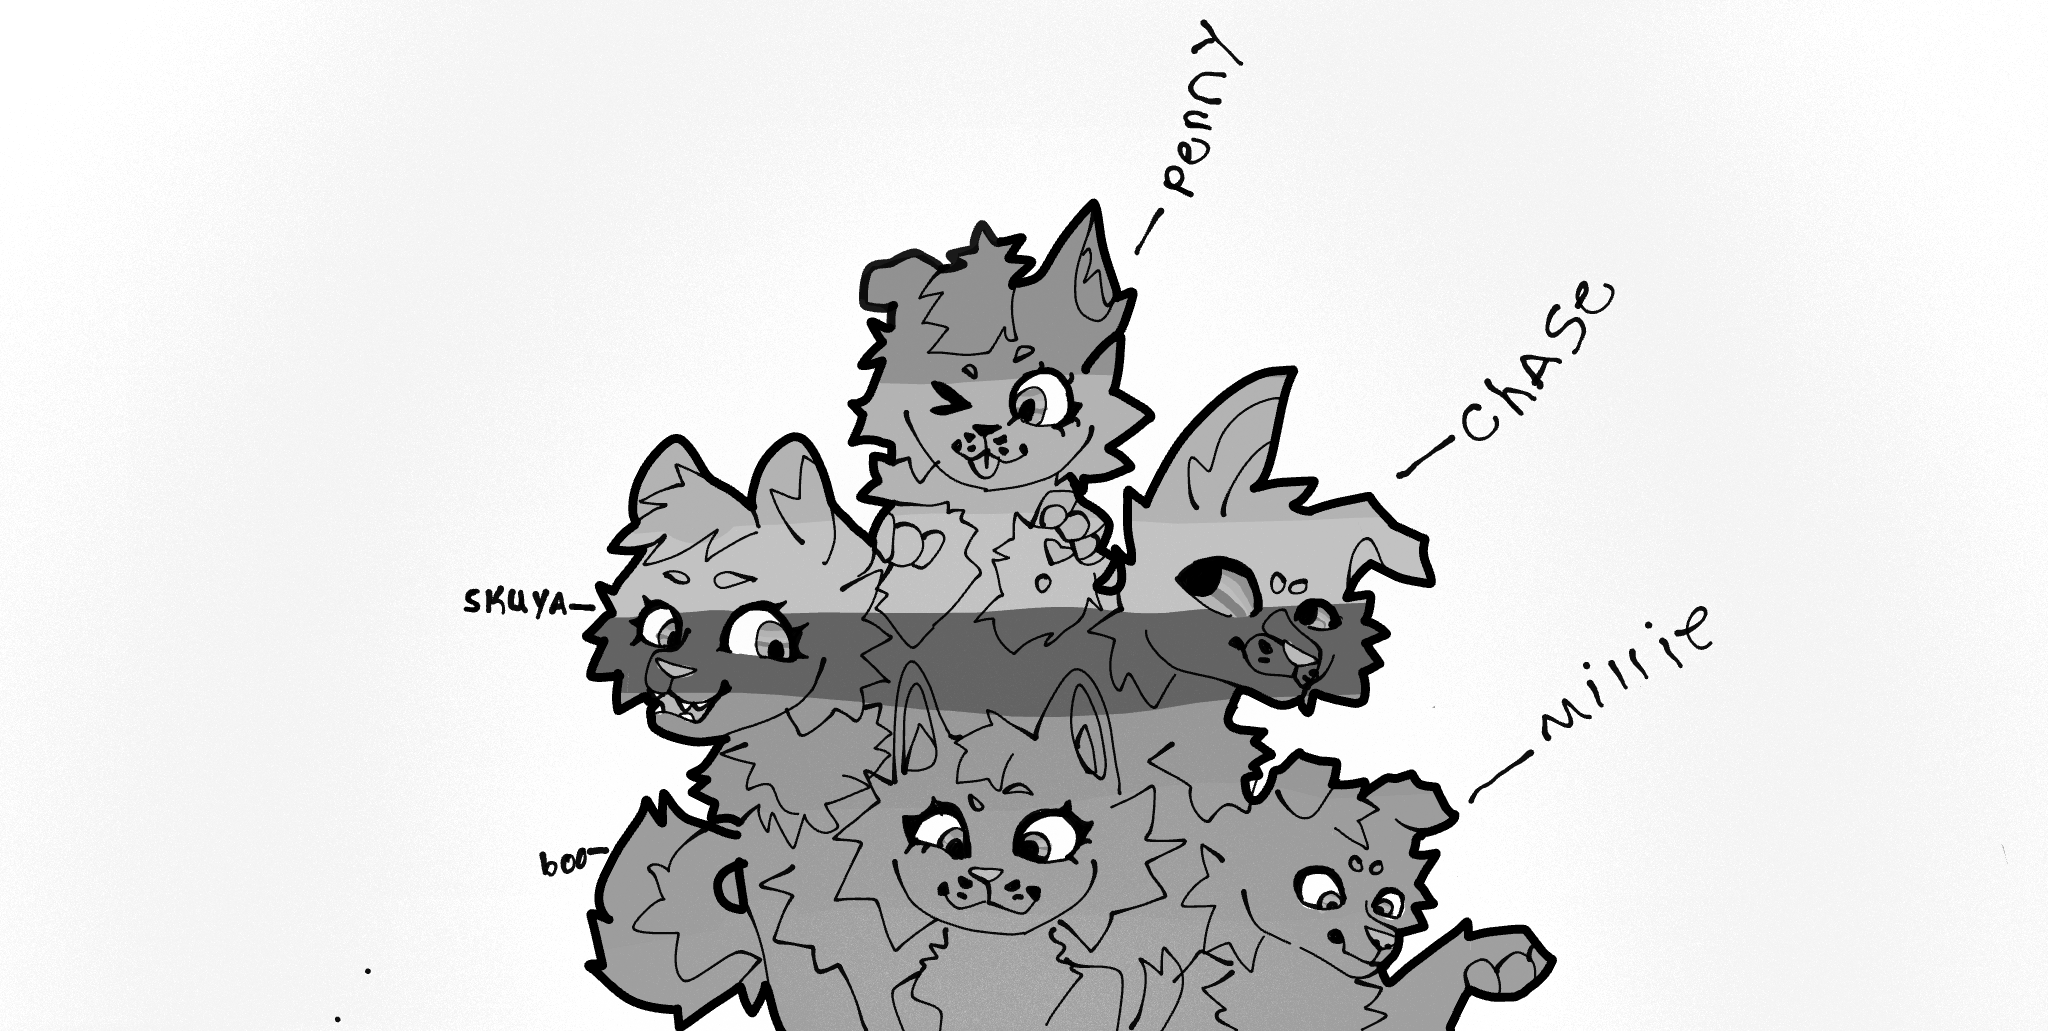
\includegraphics[width=\textwidth]{./resources/png/dream.png}
}}
\begin{center}
    \footnotesize
    \textit{An illustration of dogs that Kymberlyn chose to represent her pets}
\end{center}
\clearpage
\sectionline
\begin{center} 
\textsc{20 minutes later}
\end{center}
\;\\

She was flying! How can she fly?

“Oh no! We need to take her to the vet. Actually, they won't find anything!” I thought to myself. 
So, I searched for the drink that she drank, and it wasn't water. 
It was a flying potion. I felt terrible. She was sleeping. 
Suddenly, I remembered there was more potion on my floor, so I cleaned it up as quickly as I could. 
My Pomeranian, Skuya, got some more off my dresser and started to fly. 
When Penny woke up she wasn't flying anymore! Then, she stopped flying. 
Then, my chihuahua, Boo, got a little too. My mom asked, “Is something wrong?”

“When I took a drink, it was water, but it randomly turned to potion.” I said quickly.

“Nope, probably shouldn't have the potion on the floor!” I thought to myself.

So I cleaned it up within a flash. Most of my dogs were flying except Penny.
My mom told me that Penny was sick from the drink, she was down all day and night.
“Mom, we need to take her in.” I quickly burst out.

“No, she's fine.” Mom said sternly.

“Then I'm taking her in myself.” I said, proudly.
I quickly drove there. The vet said she had the dog flu.

\sectionline

\;\\

Two days later she was good and better. I was so glad. 
All of my dogs had stopped flying, but % and 
when I got home Penny was flying again!
“What do we do?” I asked.

“We can't do anything.” Mom assumed.

“Why?” I asked.

“It's 300 dollars, sorry.”

“Penny cant die, mom, I can't live without her!”

“I'm sorry, we can't.” Mom said.

“Goodbye Penny, I’ll miss you.”

“Wait ma'am “ said Sam.

"Yes?” I said. 

"You said it's 300 dollars?”

”yes” I answered.

"Here is 300 dollars." said Sam.

"Really!? Thank you so much!” I said.

“No problem.” Said Sam,

“Penny you're okay!” I said as I happily hugged Penny.
“Sir?” I asked.

“Yes?” said Sam.

”Here she had babies, here's a puppy.” I said.

“No, I can't take her from her mom,“ assumed  Sam.

”It's okay,” I said ”Here, thank you.”

"Welcome,” said Sam.

”Oh my god, Penny fainted! Help! Oh no.. the potion made her sick. Help someone, please!”

“Need help?” Asked Sam.

“Yes please Penny fainted!” I spoke out.

”What happened?” He asked.

“She got some kind of potion again”. I looked at the label and it was a fainting potion. 
I took her to the vet again and she was so sick that she was eating her own blood cells. 
She was only one year and three months old and she's dying.

“Why did the guy say that? I will pay for the vet bill.” Said Sam.

“No it's not your dog, it's my dog.”

“It's \$300,” The nurse said with a stern voice.

I was going home and then my dog's puppies were crying. 
I looked at one of the babies. 
It was sick and it had rabies, so we got the baby medicine and went home. 
We went to sleep then we woke up and the puppies were running around, 
so it took me an hour and a half to round them up. 
Then I put them to bed then I went to bed. 

\sectionline

\;\\

After they were done I woke up and I was sick, so I went to the hospital. 
The puppies were in my car when I went to the emergency room. 
When I was done the car was a total mess so I had to put a puppy in time out. 
After she went into timeout she was sad and 
she was in a corner that she couldn't go in so she was mad. 
The floor was wet from her peeing and I was so mad at her 
that I did nothing and let my mom do it. I went to my room.

“Kymber come clean up your dog's pee,”

“No mom,” I said.

“She's yours.” Mom commented.

“Ugh, fine.”  said angrily.

“Go to your room, Kymber.”

“Why mom?”

“Because I said!”

“Fine mom, come on Penny. Good night Penny.” 
The next morning we went to the pet store so she could get treats. They were out!

“Penny, come on.” We went to another pet store. The treats weren't there either.

“Huh, weird. Penny, let's go home.” When we got home we saw a cat at the door.

“Huh, where did you come from cutie?” The cat attacked Penny! I had to take her to the vet again.

“Ugh, what's wrong with Penny?” The vet asked. Penny barked in sadness.

“Oh, Penny, you're okay. I’m here.” I told Penny.

“She needs surgery fast!” the Vet said. “I don't have money.” I told Sam.

“Okay, I'll pay for it.” Sam said.

“Thank you so much!” I said happily.

“Of course I'm here for Penny.” said Sam, “Okay, let's get Penny into surgery.”

“Okay! Come on.” Penny whines.

“It's okay Penny.” I said.

“She’s okay. The surgery was good.”

“Thank god.” 

I woke up from my dream and screamed "Penny! Where are you?” 

Penny came running in the room. “Ruff?” We went to sleep. 
Then my grandma's dog Millie May was laying next to me. 
And we were all asleep again

\chapterline{Black}{88}
\begin{center}
  \;\\{
  \fbd
  \fbox{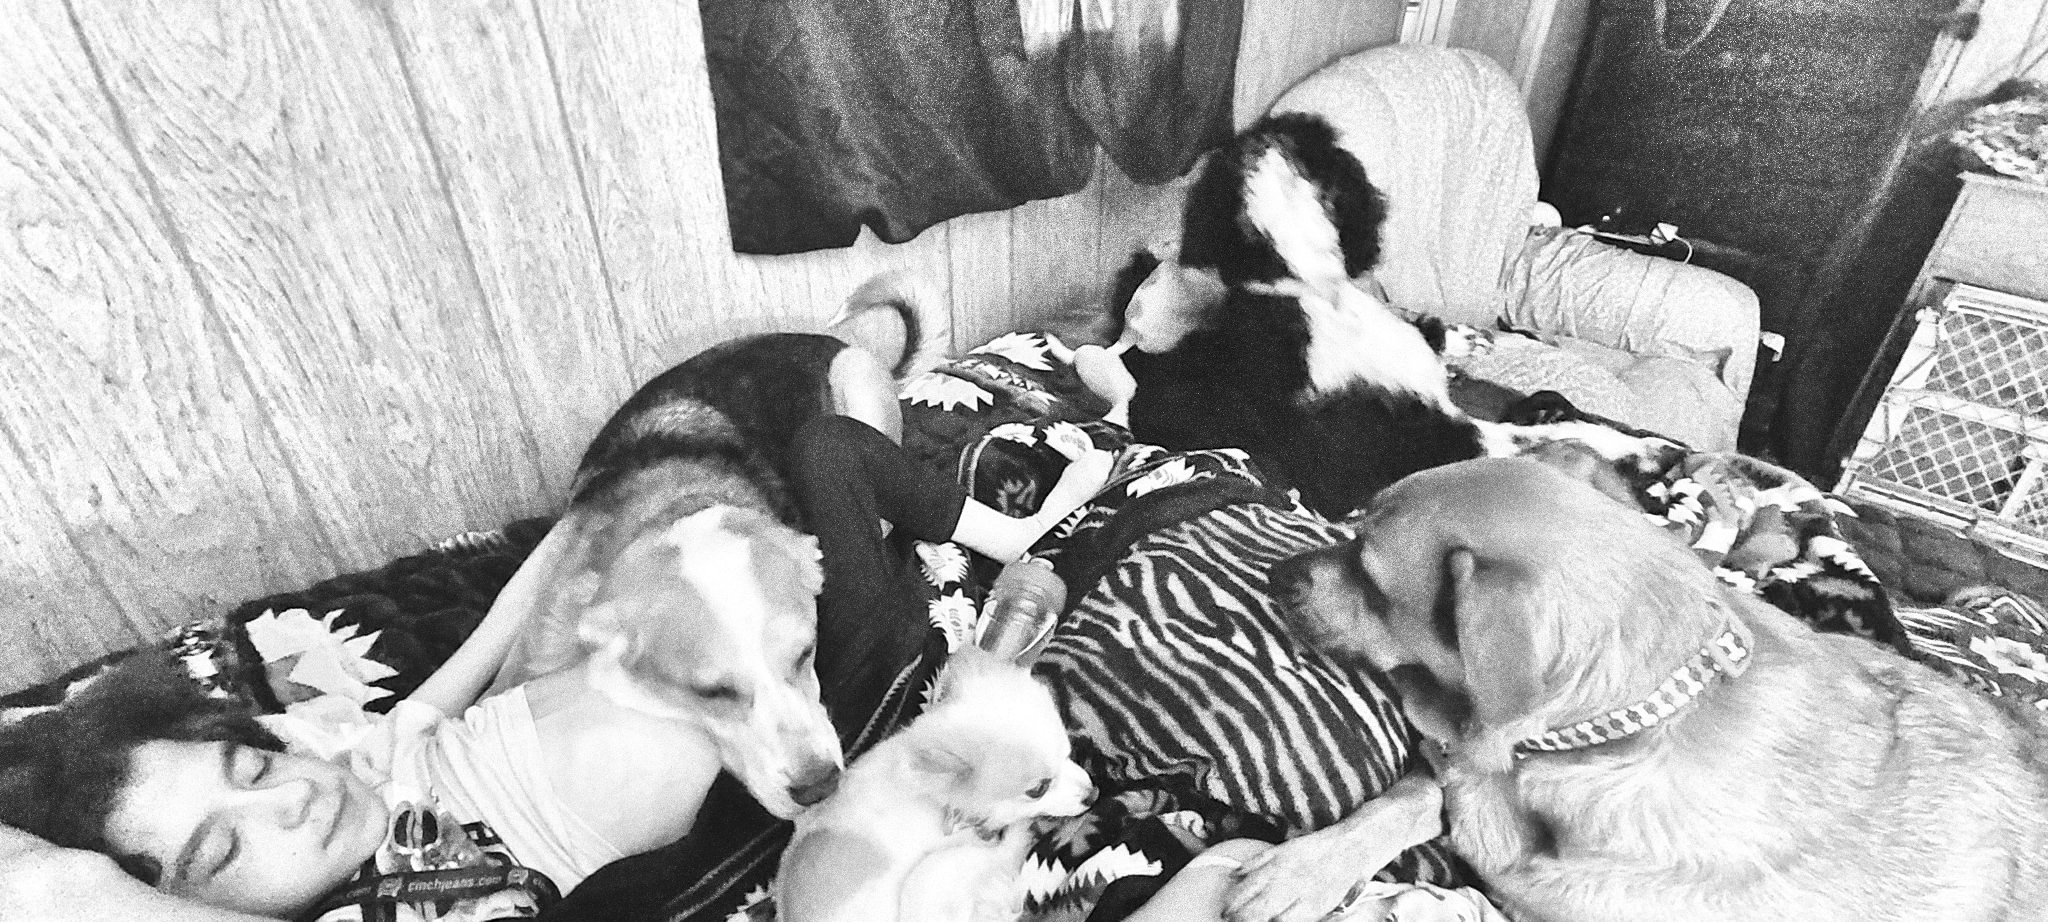
\includegraphics[width=\textwidth]{./resources/png/fur-babies.png}
  }}
  \footnotesize\;\\
  \textbf{Kymberlyn and her Fur Babies}
  \;\\
  \;\\{
    \fbd
    \fbox{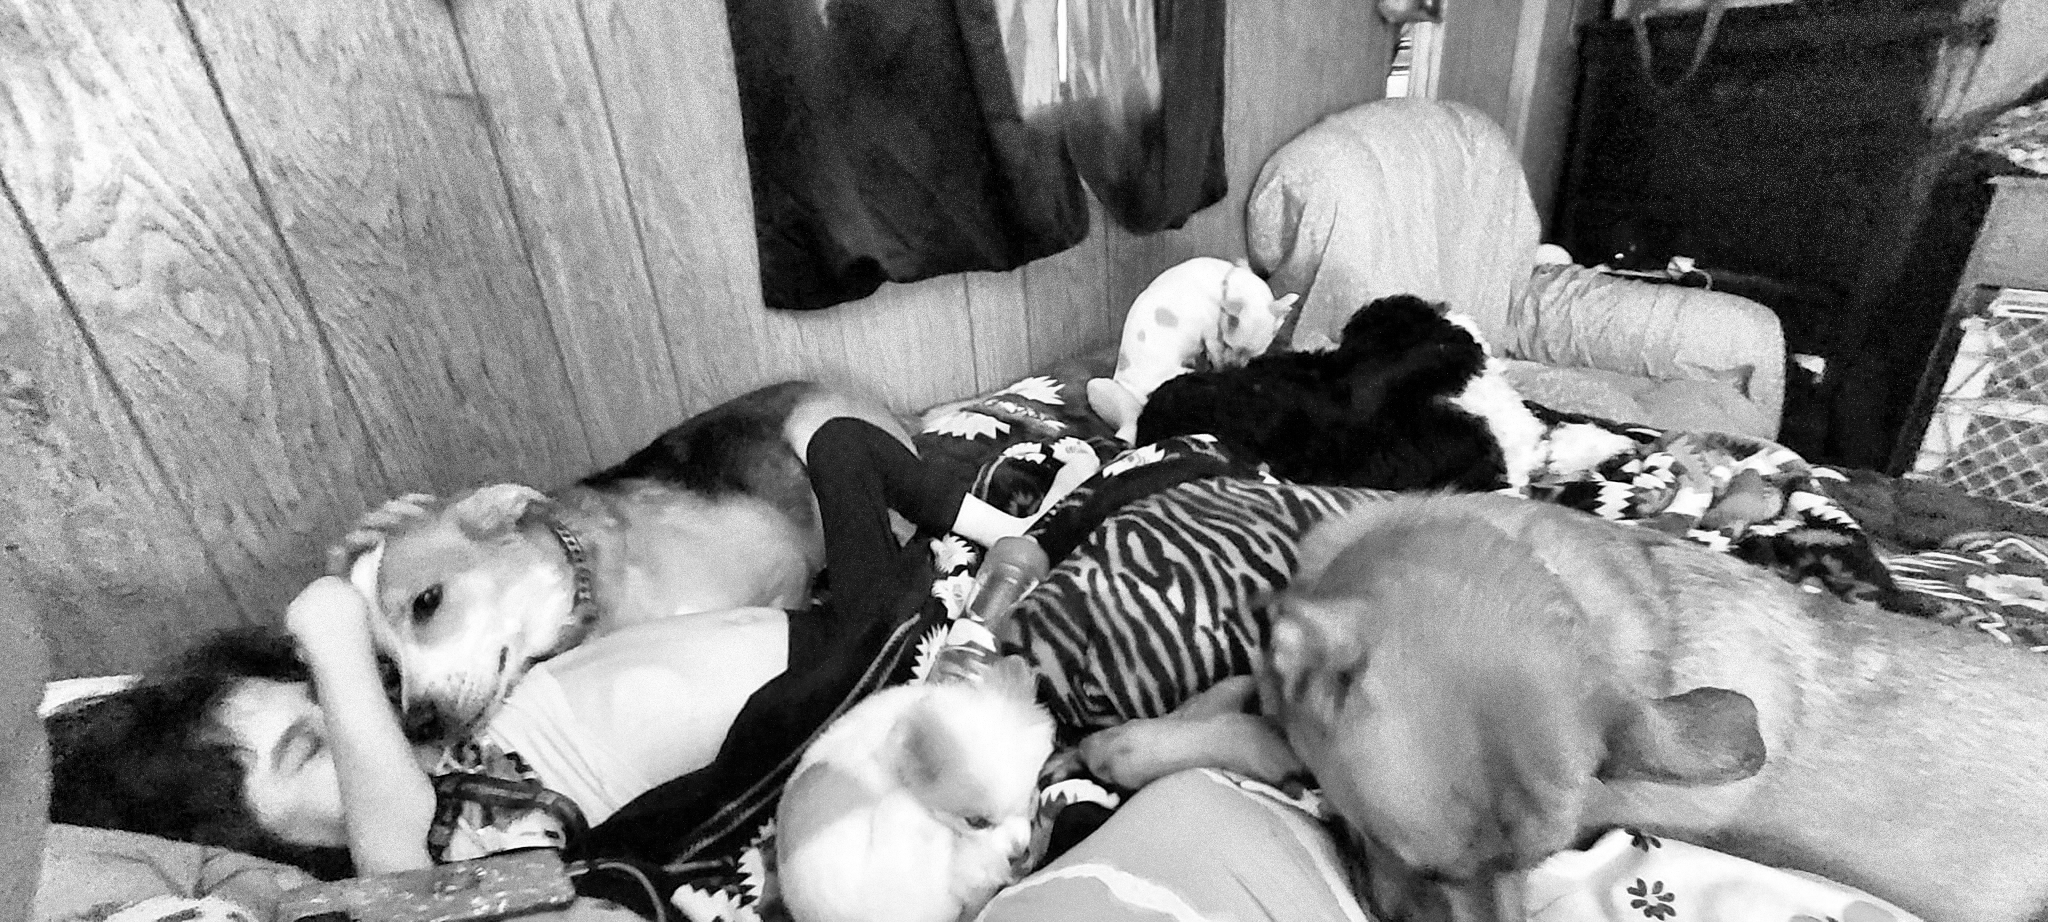
\includegraphics[width=\textwidth]{./resources/png/fur-babies-2.png}
  }}
\end{center}






\clearpage




%%%%%%%%%%%%%%%%%%%%%%%%%%%%%%%%%%%%%%%%%%%%%%%%%%%%%%%%%%%%%%%%%%%%%%%%%%%%%%%%
%%%%%%%%%%%%%%%%%%%%%%           CHAPTER TWO          %%%%%%%%%%%%%%%%%%%%%%%%%%
%%%%%%%%%%%%%%%%%%%%%%%%%%%%%%%%%%%%%%%%%%%%%%%%%%%%%%%%%%%%%%%%%%%%%%%%%%%%%%%%

\chapter*{%
  \huge An Autobiographical Poem\\
  \small \;\\by Kymberlyn Davis
}

\begin{center}
  \texttt{
    Kymberlyn\\
    caring, cute, silly\\
    fan of my boyfriend, friends, myself\\
    who feels happy, scared, sad\\
    boyfriend, family, and Logan my friend\\
    My mom provides for my brother and I\\
    I'm scared of getting heartbroken and spiders\\
    My boyfriend and family want to see\\
    Alaska, Colorado, Texas\\
     Davis
    }
    \;\\
    \;\\
    \;\\{%
      \fbd
    \fbox{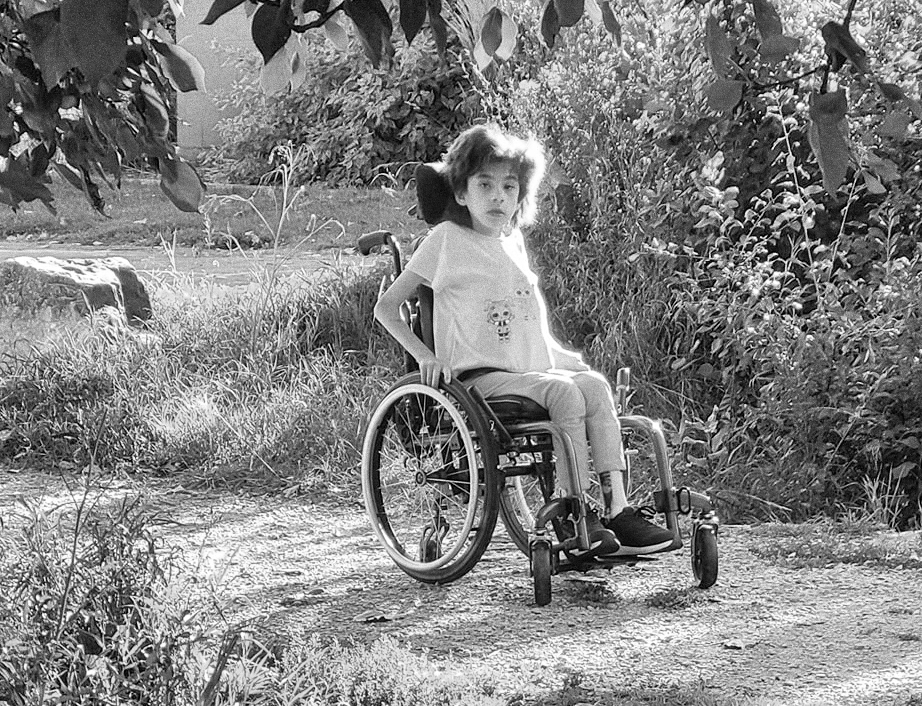
\includegraphics[width=0.85\textwidth]{./resources/png/bio-poem.png}}}
\end{center}
\clearpage



%%%%%%%%%%%%%%%%%%%%%%%%%%%%%%%%%%%%%%%%%%%%%%%%%%%%%%%%%%%%%%%%%%%%%%%%%%%%%%%%
%%%%%%%%%%%%%%%%%%%%%%           CHAPTER THREE        %%%%%%%%%%%%%%%%%%%%%%%%%%
%%%%%%%%%%%%%%%%%%%%%%%%%%%%%%%%%%%%%%%%%%%%%%%%%%%%%%%%%%%%%%%%%%%%%%%%%%%%%%%%

\chapter*{%
  \huge Different\\
  \small \;\\ A Poem by Kymberlyn Davis
}

\begin{verse}
\poemlines{2}

\begin{altverse}
How are we so "different"?\\
  If different is just a thing\\
If we all have certain features\\
  What does different bring?\\!


People filled with hatred\\
  Can't possibly see\\
There's not really differences\\
  Between me and you\\!

  
Looks can't show difference\\
  If they're just there to be seen\\
If you don't look like someone else\\
  Why are they so mean?\\!


If being different\\
  Is what is wrong,\\
I'd rather not be right\\
  And I'd want to finish living.\\!    
\end{altverse}
\end{verse}

\begin{center}
    \tiny \;\\\;\\{%
      \fbd
    \fbox{\includegraphics[width=0.55\textwidth]{./resources/png/different.png}}}
\end{center}

\clearpage


%%%%%%%%%%%%%%%%%%%%%%%%%%%%%%%%%%%%%%%%%%%%%%%%%%%%%%%%%%%%%%%%%%%%%%%%%%%%%%%%
%%%%%%%%%%%%%%%%%%%%%%           CHAPTER FOUR         %%%%%%%%%%%%%%%%%%%%%%%%%%
%%%%%%%%%%%%%%%%%%%%%%%%%%%%%%%%%%%%%%%%%%%%%%%%%%%%%%%%%%%%%%%%%%%%%%%%%%%%%%%%

\chapter*{%
  \huge All About Me\\
  \small \;\\Adapted from a presentation by Kymberlyn Davis
}
\section*{Introduction}{%
  \fbd
  \fbox{
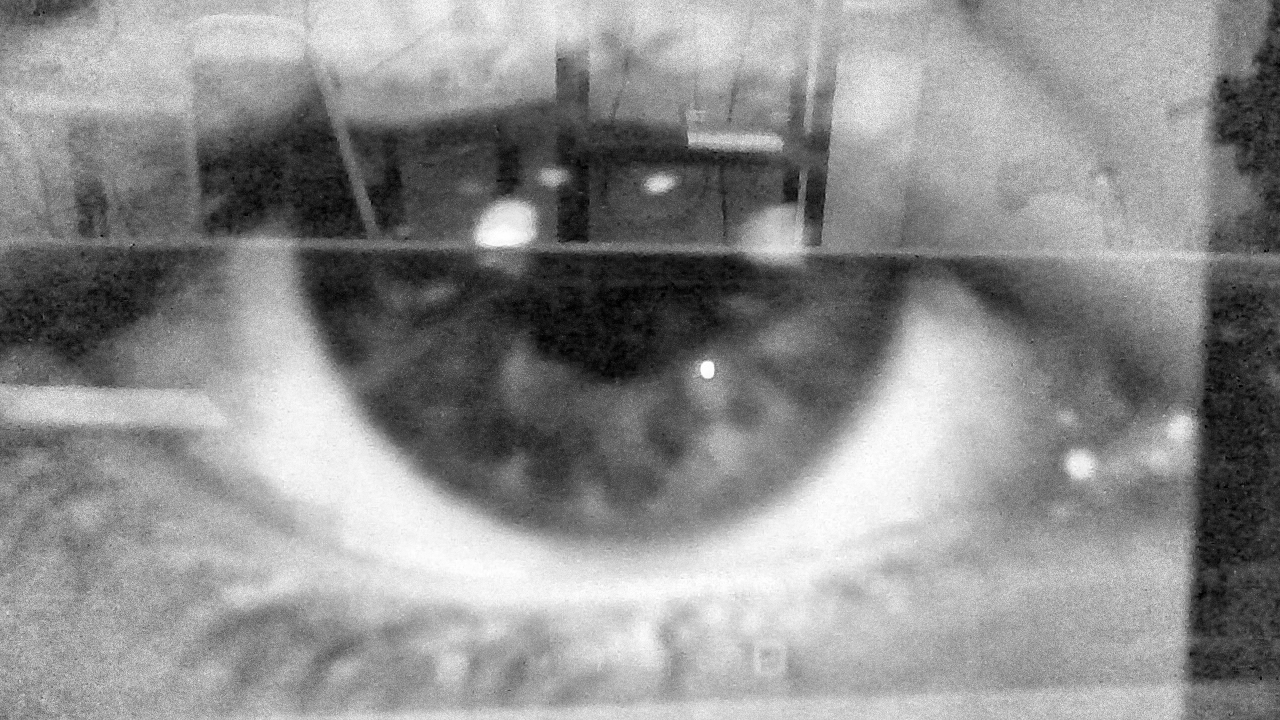
\includegraphics[width=\textwidth]{./resources/png/eye.png}
}}
\;\\
Hi, this is me. My name is Kymberlyn Davis\\
My date of birth is December 20, 2011;\\
I'm 4ft 1in tall and have hazel eyes and I'm 12 years old\\
i was named after my grandma and great grandmother\\
my grandmas name is kimberly\\
my middle name is from my great grandmother its clara lee\\
and my last name is davis \\
my  nicknames are kym, kymber, kymberly and kym\\
I live in Rapid City and was born here\\
I live in a house and it's cool.
\clearpage
\section*{My Family}{
  \fbd
  \fbox{
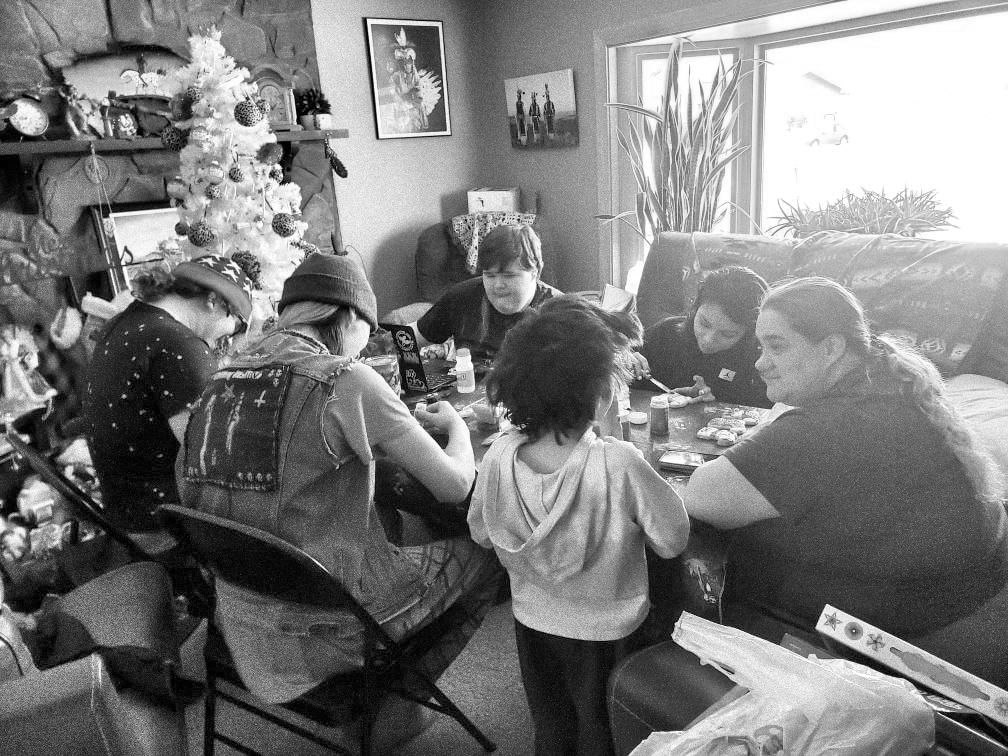
\includegraphics[width=\textwidth]{./resources/png/family.png}
}}
\;\\
I live in a home of three: me, my mom, and my brother Chance.\\
My mom has brown hair and hazel eyes like me. \\
She's nice, loving, and sweet.\\
My brother has brown hair and brown eyes. \\
He's mean funny and inappropriate.\\
My sister is a scientist and she has green eyes. \textit{[blue]}\\
She's getting married to her girlfriend Lydia,\\
who has brown and green hair and she is my stepsister \textit{[Sister-in-Law]}\\
My  grandma is my life.
She's sweet and loving and I'm her favorite.\\
My aunt Leslie lives with my grandma.\\
She's nice, sassy, and thinks of other people.\\
My aunt Desire\'e shes a really nice aunt and I am happy to be here writing this\\
My dad hes nice and kind he works for oil.
\clearpage
\section*{My Friends}{%
  \fbd
  \fbox{
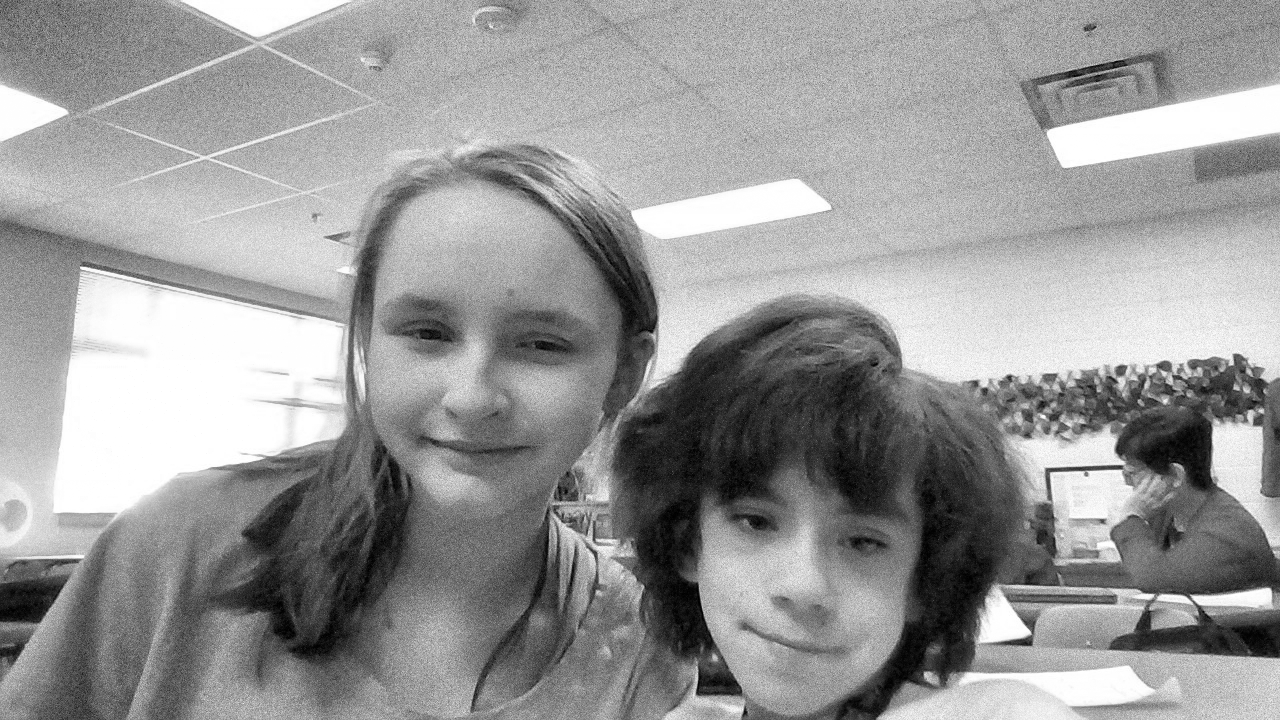
\includegraphics[width=\textwidth]{./resources/png/friends.png}
}}
\;\\
My friends are Araya, Kloe, Crysta, Aurora, and Noah.\\
My girlfriends were Payton Kester and Anna Kemp, but they aren't anymore\\
\clearpar
\section*{My Life and the Things I Like}
\begin{minipage}{0.45\linewidth}
I like Chef Boyardee Homemade Pizza\\
My favorite movies are Grown Ups and the My Little Pony movie.\\
I really want to go to Hawaii.\\
My favorite songs are "Without Me", "Broken", "10 Things I Hate About You",
"Attention", "IDFC", and "If I Would Have Known"\\
I like wolves, cats, dogs, foxes, and axolotls.\\
I like art, cooking, and math\\
I love listening to music and chilling\\
I don't like English class.\\
\end{minipage}
\begin{minipage}{0.45\linewidth}
  \hfill
  {\fbd
  \fbox{
  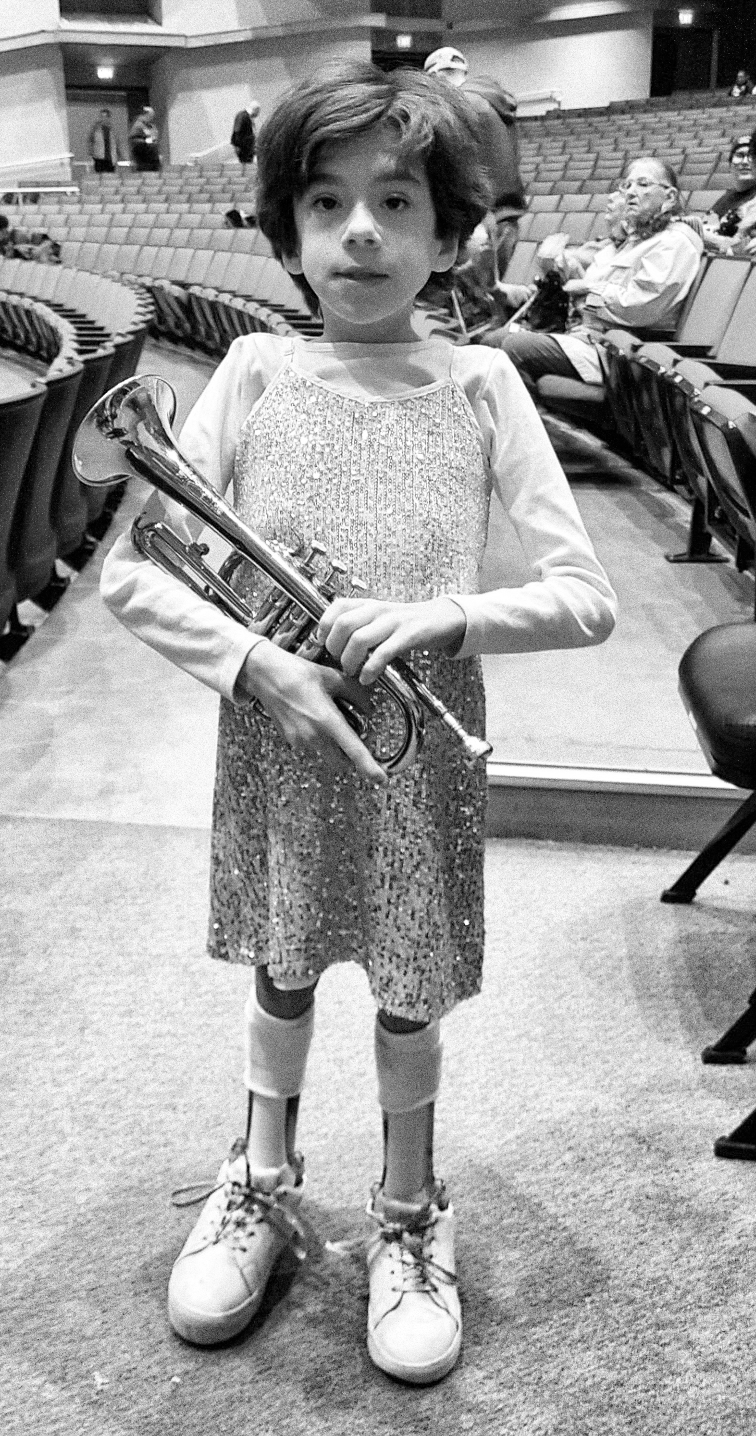
\includegraphics[width=0.7\textwidth]{./resources/png/music.png}
  }}
\end{minipage} 
\clearpage
\section*{Things I'm Scared Of}
\begin{minipage}{0.45\linewidth}
I'm scared of zombies and anything creepy\\
I have no \textbf{F}'s in my grades and I'm really good at math.\\
\end{minipage}
\begin{minipage}{0.45\linewidth}
  \hfill
  {\fbd
    \fbox{
  \includegraphics[width=0.85\textwidth]{./resources/png/fridge.png}
  }}
\end{minipage}

\section*{Memories}
\begin{minipage}{0.45\linewidth} 
On January 11$^{th}$, 2023 I got a baby puppy and I was so happy I was in
love with her\\
Her name is Penny. \\
Her nicknames are Lulu and Penpen.\\
\;\\
I want to be a singer or a doctor, have a boyfriend, and live in a house.\\
I want two kids and I'll be happy
\end{minipage}
\begin{minipage}{0.45\linewidth}
  \hfill
  {\fbd
    \fbox{
  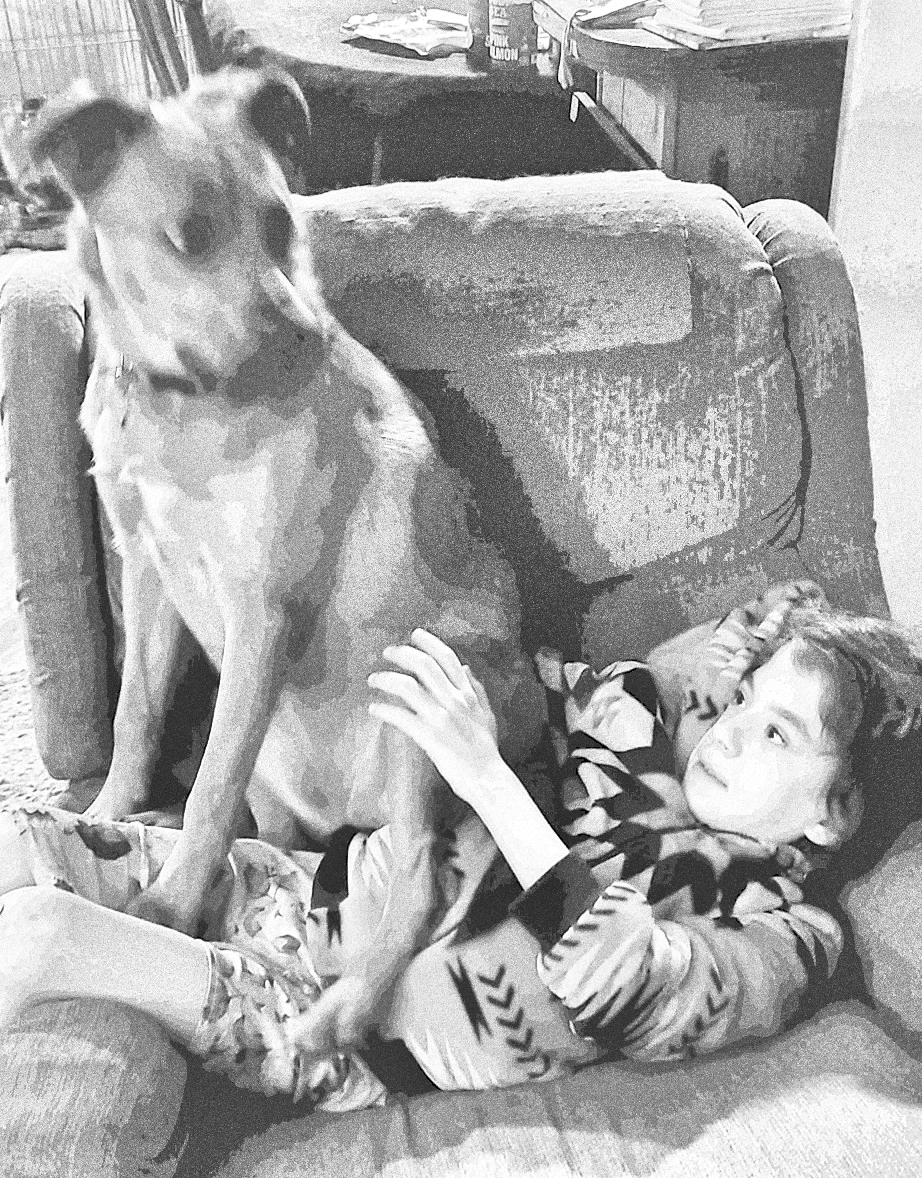
\includegraphics[width=0.85\textwidth]{./resources/png/penny.png}
}}
\end{minipage}


\section*{Special Things}
I've had 20 surgeries and I've traveled to Minnesota over 20 times.\\
I'm really good at being a soccer goalie.\\
I'm very loved
\begin{center}
  {\fbd
    \fbox{
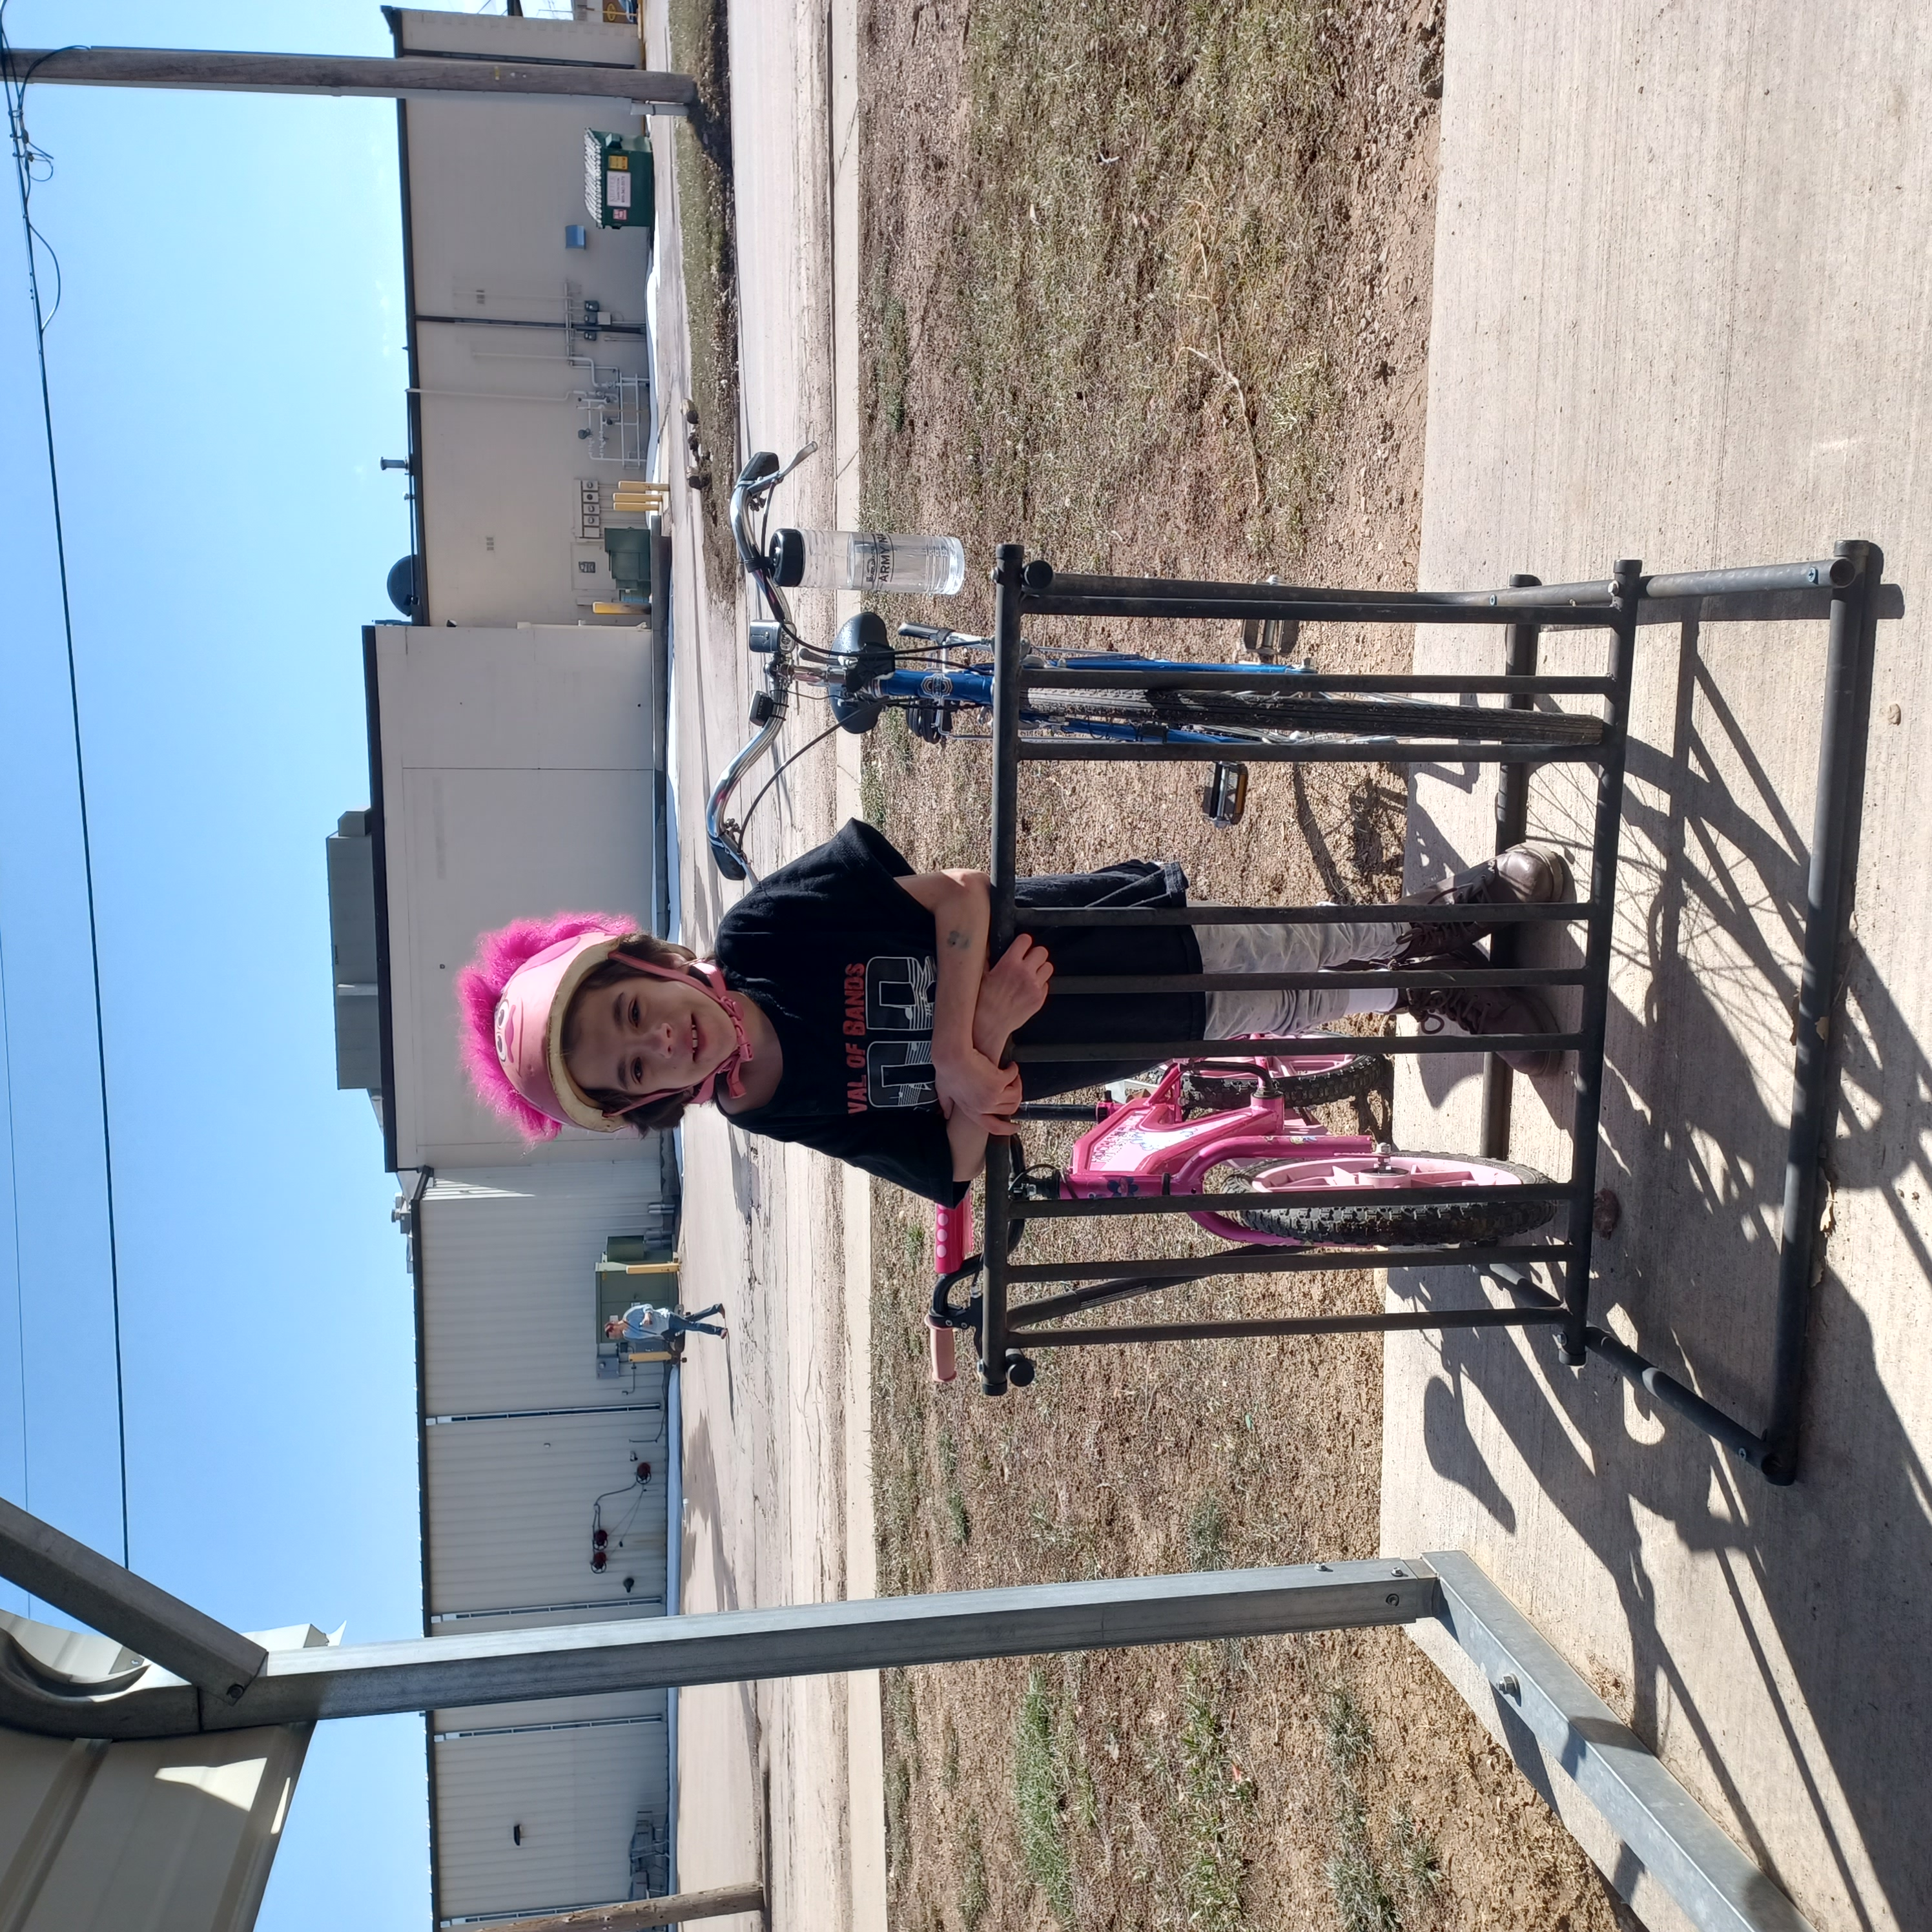
\includegraphics[width=0.5\textwidth]{./resources/png/bike.png}
}}

  \textbf{Kymberlyn knew she was very loved.}
\end{center}

\clearpage
%%%%%%%%%%%%%%%%%%%%%%%%%%%%%%%%%%%%%%%%%%%%%%%%%%%%%%%%%%%%%%%%%%%%%%%%%%%%%%%%
%%%%%%%%%%%%%%%%%%%%%%           CHAPTER FIVE         %%%%%%%%%%%%%%%%%%%%%%%%%%
%%%%%%%%%%%%%%%%%%%%%%%%%%%%%%%%%%%%%%%%%%%%%%%%%%%%%%%%%%%%%%%%%%%%%%%%%%%%%%%%

\chapter*{Kymberlyn's Obituary}
\lettrine{\fbox{\usefont{U}{Zallman}{xl}{n}K}}{  }
ymberlyn Clara Lee Davis was a 12 year old lovable and sassy pre-teen who loved
school, her family, her friends, and her dogs.  

She had a long history of medical issues and diagnosis,
which left her vulnerable and with a compromised immune system. 

Kymberlyn was born 6 weeks premature at Monument Hospital on December 20, 2011
to Jamie Lynn Davis and Jon Joseph Wagner. 

She attended Robbinsdale Elementary school and went on to East Middle School
where she attended 6th grade. 

Kymberlyn enjoyed many things, including cooking, Girl Scouts,
drawing and coloring, going out for ice cream, helping her mom clean the house,
traveling, and her five dogs. She was active on Tik-Tok, Snapchat, Youtube, and
Roblox, and she played video games. She also liked Yatzee and Skipbo. 

Kymberlyn had many friends world wide and loved everyone
she met as much as they loved her. 

Grateful for having shared her life are her mother, Jamie; 
father, Jon; her two brothers, Ryott and Chance; 
grandmother, Kimberly Davis; aunts, Leslie and Desiree Davis; 
and many cousins, great aunts and uncles, 
and all of her extended family and friends who will miss her dearly. 

Kymberlyn is preceded in death by her grandparents, James Davis, 
Duane and Barbara Wagner; and many cousins, aunts, and uncles. 

She passed on March 12, 2024 at 01:11\textsc{am}, surrounded by her family.

Her service is on March 21, 2024 at the Shrine Center in Rapid City.
\clearpage

%%%%%%%%%%%%%%%%%%%%%%%%%%%%%%%%%%%%%%%%%%%%%%%%%%%%%%%%%%%%%%%%%%%%%%%%%%%%%%%%
%%%%%%%%%%%%%%%%%%%%%%           CHAPTER FIVE         %%%%%%%%%%%%%%%%%%%%%%%%%%
%%%%%%%%%%%%%%%%%%%%%%%%%%%%%%%%%%%%%%%%%%%%%%%%%%%%%%%%%%%%%%%%%%%%%%%%%%%%%%%%

\begin{center}
  \;\\
  \;\\
  \;\\
  \;\\
  \;\\
  {\fbd
    \fbox{
  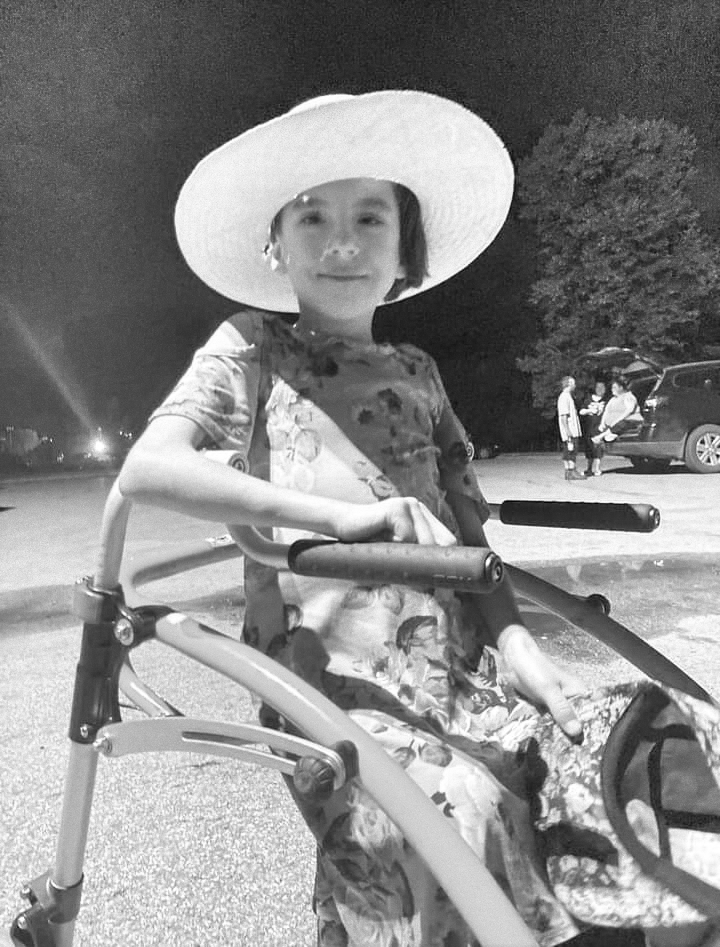
\includegraphics[width=\linewidth]{./resources/png/kymberlyn.png}
}}

  \textbf{Published in loving memory of Kymberlyn Clara Lee Davis}
\end{center}



\end{document}
